\documentclass[10pt]{beamer}

%%%
% PREAMBLE FOR THIS DOC 
%%%
%https://tex.stackexchange.com/questions/68821/is-it-possible-to-create-a-latex-preamble-header
\usepackage{/Users/miw267/Repos/csci246_spring2025/slides/preambles/beamer_preamble_for_CSCI246}


%%% TRY TO RESHOW TOC AT EACH SECTION START (with current section highlighted)
% Reference: https://tex.stackexchange.com/questions/280436/how-to-highlight-a-specific-section-in-beamer-toc
\newcommand\tocforsect[2]{%
  \begingroup
  \edef\safesection{\thesection}
  \setcounter{section}{#1}
  \tableofcontents[#2,currentsection]
  \setcounter{section}{\safesection}
  \endgroup
}


%%%% HERES HOW TO DO IT CORRECTLY
% FIRST IN .STY FILE, DO
%\usetheme[sectionpage=none]{metropolis}
% THEN AT EACH SECTION DO
%\begin{frame}{Outline}
%  \tableofcontents[currentsection]	
%\end{frame}



%\setbeamertemplate{navigation symbols}{}
%\setbeamertemplate{footline}[frame number]{}


%%%
% DOCUMENT
%%%

\begin{document}

%\maketitle

%% Title page frame
%\begin{frame}
%    \titlepage 
%\end{frame}



\title{04/07/2025: Algorithm Efficiency}
\author{CSCI 246: Discrete Structures}
\date{Textbook reference: Sec 11.3, Epp}

\begin{frame}
    \titlepage 
\end{frame}


\begin{frame}
\small
\begin{mygreenbox}[title=Graded Quiz Pickup]
Quizzes are in the front of the room, grouped into four bins (A-G, H-L, M-R, S-Z) by last name. The quizzes are upside down with your last name on the back. Come find yours before, during, or after class. Only turn the quiz over if it's yours.
\end{mygreenbox} 
\vfill 
%\begin{myredbox}[title=Friday's Problems Quiz]
%The problems quiz on Friday (04/02) will cover:
%\begin{itemize}
%\item Conditional Probability and Independence
%\item Random Variables
%\item Expectations	
%\end{itemize}
%
%\end{myredbox}
\vfill 
\begin{myyellowbox}[title=Today's Agenda]
\begin{itemize}
	\item Reading quiz (5 mins)
	\item Mini-lecture ($\approx$ 15 mins)
	\item Group exercises ($\approx$ 20 mins)
\end{itemize}


\end{myyellowbox}
\vfill 

\end{frame}






\begin{frame}[standout]
Feedback on Friday's Quizzes
\end{frame}

\begin{frame}{Problem Quiz Scores}
\small 
\begin{figure}[ht]
        \centering
        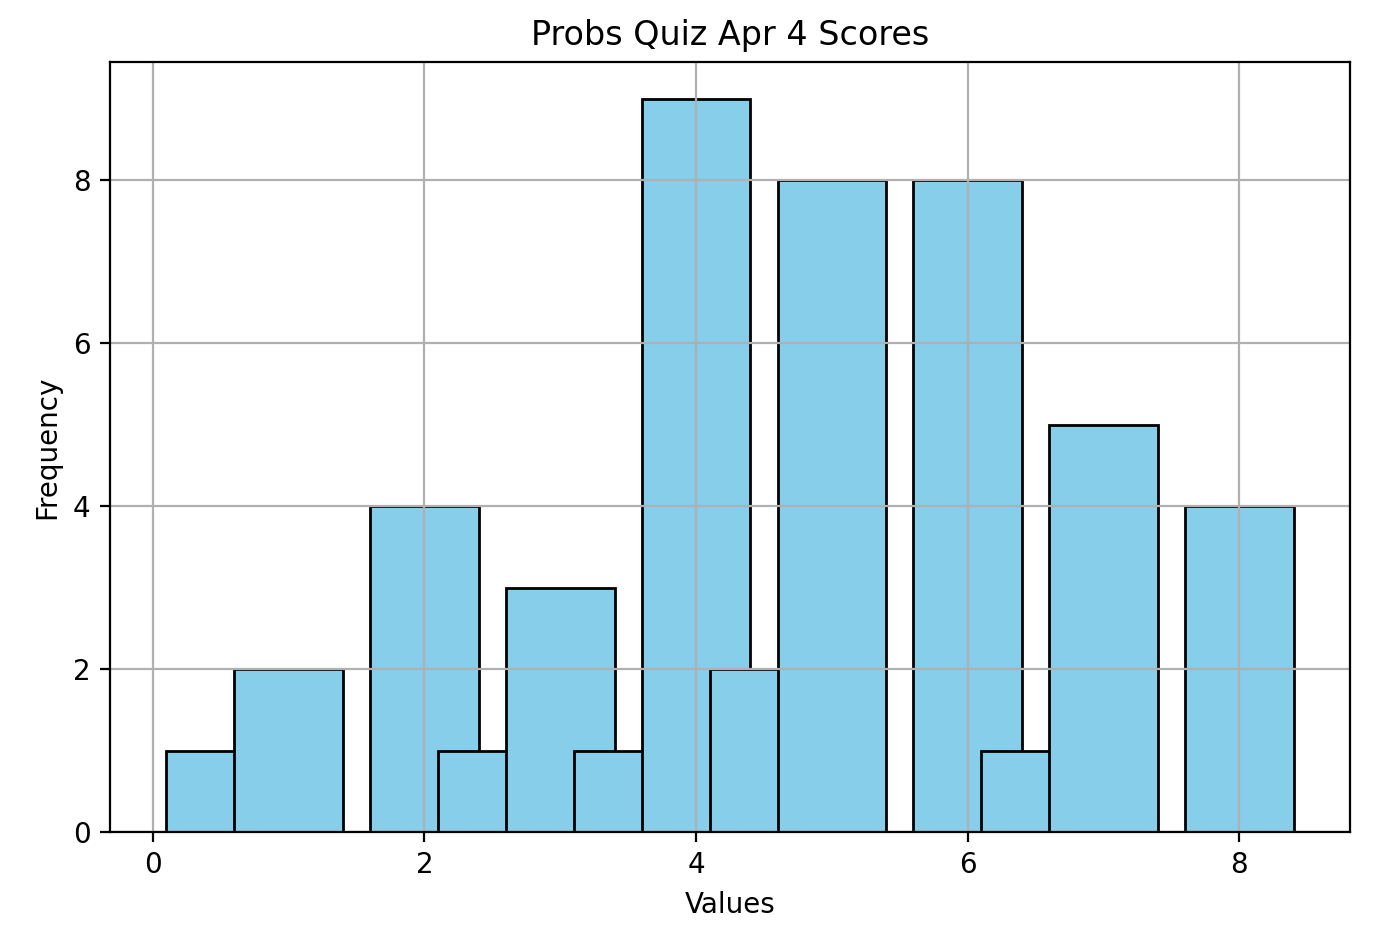
\includegraphics[width=.6\textwidth]{images/problem_quiz_scores}
   		 \caption{Median Score = 5/8 (62.5\%)}
\end{figure}
\vfill 
\vspace{-.3cm}
\textbf{Grading Rubric:}  
\begin{enumerate}
	\item (4 points.) 2 points for $P(A|B)$ and 2 for $P(B|A)$.  Must show work for full credit. 
	\item (4 points.) 1 point for correct answer,  1 point for stating correctly one of the 3 characterizations of independence, 2 points for correctly determining the probabilities needed for that characterization.  
\end{enumerate}(4 points.) 


\end{frame}	

\begin{frame}{Reading Quiz Scores (Extra Credit)}
\begin{figure}[ht]
        \centering
        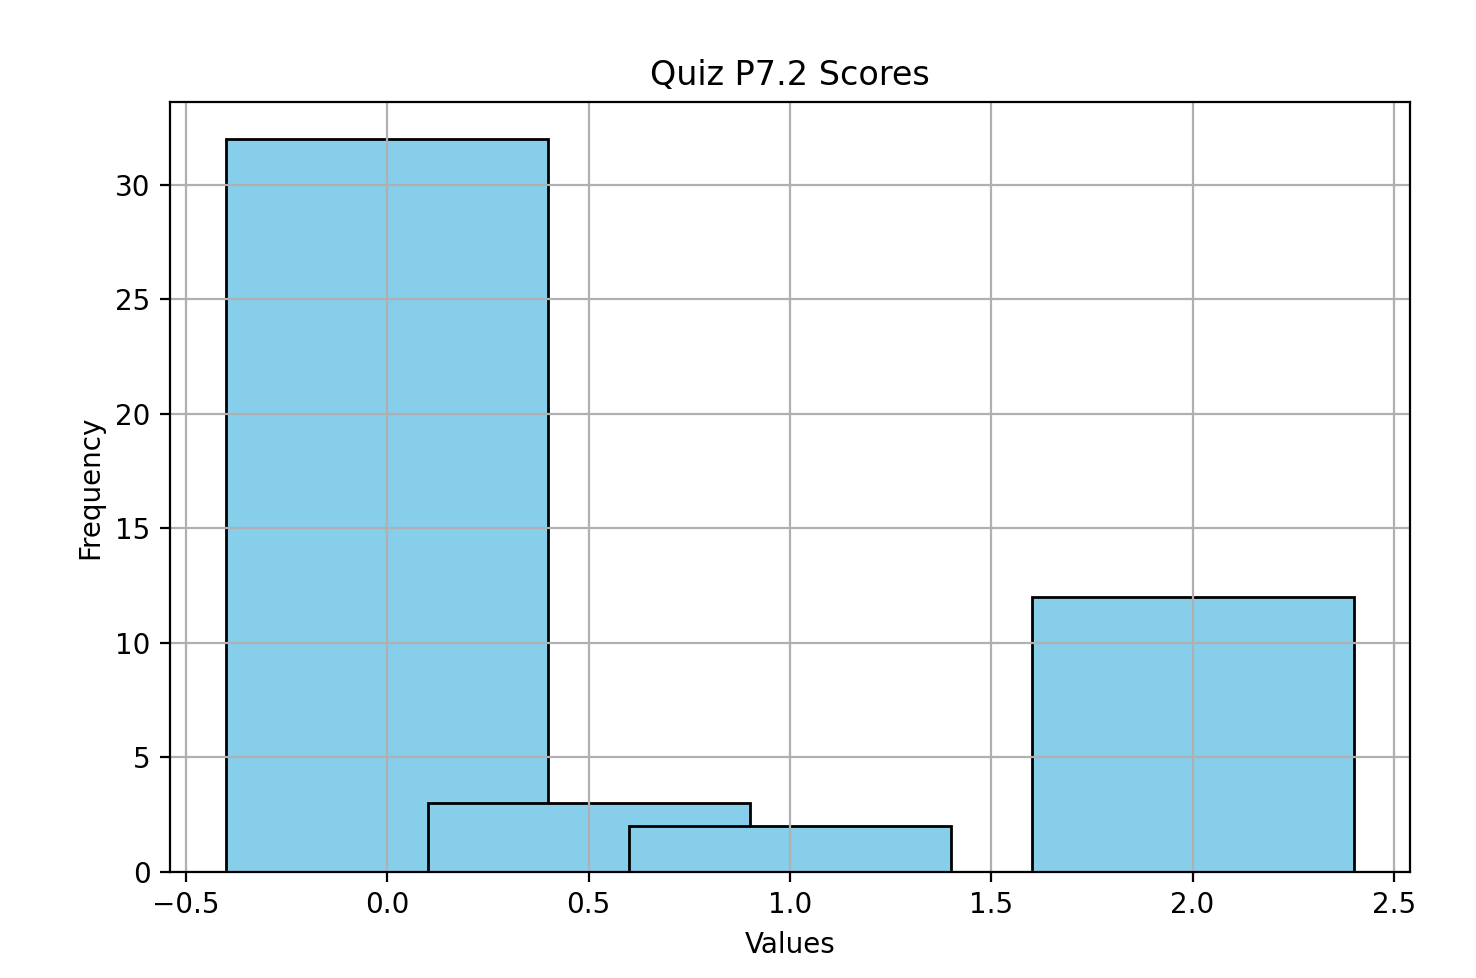
\includegraphics[width=.7\textwidth]{images/reading_quiz_scores}
   		 \caption{Median Score = 0 points extra credit}
\end{figure}
\vfill 
\textbf{Grading Rubric:}  2 points extra credit for perfect answer.
\end{frame}	




\begin{frame}[standout]
Today's reading quiz
\end{frame}

\begin{frame}
\small 
\begin{myredbox}[title=Reading Quiz (Algorithm Efficiency)]
Assume $n$ is a positive integer and consider the following algorithm segment:
\begin{figure}
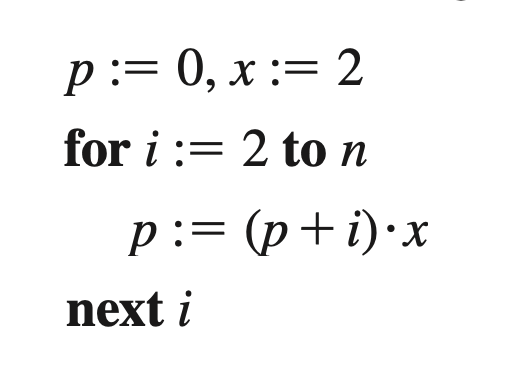
\includegraphics[width=.6\textwidth]{images/algorithm_segment.png}	
\end{figure}
\begin{enumerate}
	\item What is the actual number of elementary operations that are performed when this algorithm segment is executed? Justify your answer.
	\item What is the order for this algorithm segment? Justify your answer.
\end{enumerate}
\end{myredbox}
\end{frame}


\begin{frame}[standout]
Review of Problems Quiz
\end{frame}



\begin{frame}[standout]
Thoughts On Algorithm Efficiency
\end{frame}

\begin{frame}

\begin{mygreenbox}[title=\text{Theorem: Sum of the first $n$ natural numbers}]

For every natural number $n \geq 1$, 
\[ 1 + 2 + \cdots + n = \frac{n \, (n+1)}{2} \]
\end{mygreenbox}

\vfill 
\pause 
\begin{myredbox}[title=\text{Story: Gauss' solution from elementary school}]
\begin{figure}
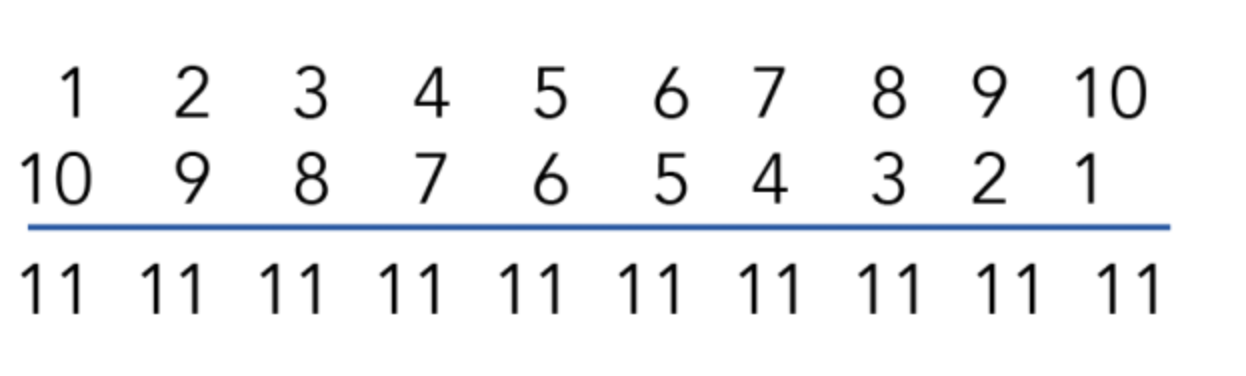
\includegraphics[width=\textwidth]{images/gauss_sum.png}	
\end{figure}	
\end{myredbox}
\end{frame}



\begin{frame}[fragile]

\colorbox{yellow!30}{\textbf{Poll.}} How does the theorem apply to algorithm efficiency?
\pause 
\vfill 
\colorbox{green!30}{\textbf{Solution.}} Consider an algorithm segment with a nested for loop, such as the one below.

\begin{myredbox}[title=\text{An algorithm segment with a nested for loop}]
\begin{lstlisting}
for i = 1 to n:
    for j = 1 to i:	
      	print "YOLO"
\end{lstlisting}
\end{myredbox}
\vfill 
\pause 

The number of times the inner loop is run is 
\[1+2+3+4+ \hdots + n \]

We need this quantity to compute algorithmic efficiency, since the number of elementary operations performed by an algorithm segment is given by
\[ \#  \text{elem. ops} \; = \; \#  \text{inner loops}   \; \times \; \#  \text{elem. ops. per inner loop} \]

\end{frame}

\begin{frame}{Remark: Big O is not worst case}

\begin{columns}[c]
    \column{0.4\textwidth}
    \centering
    \textbf{Method for computing} \\
    \textbf{\# elem. operations} \\
    Worst Case \\
   	Best Case  \\
	Average Case

    \column{0.1\textwidth}
    \centering
	{\Huge $\times$}
    
    \column{0.5\textwidth}
    \centering
    \textbf{Method for expressing} \\
    \textbf{order of algorithm} \\
    Big O \\
   	Big Theta  \\
	Big Omega

\end{columns}
	
\end{frame}


\begin{frame}[standout]
Group exercises
\end{frame}

\begin{frame}
\footnotesize 
\vfill 
\begin{columns}
\begin{column}{0.33\textwidth}
aaron.loomis: 5 \\ 
adam.wyszynski: 6 \\ 
alexander.goetz: 18 \\ 
alexander.knutson: 6 \\ 
anthony.mann: 20 \\ 
blake.leone: 16 \\ 
bridger.voss: 14 \\ 
caitlin.hermanson: 12 \\ 
cameron.wittrock: 3 \\ 
carsten.brooks: 1 \\ 
carver.wambold: 4 \\ 
colter.huber: 20 \\ 
conner.reed1: 7 \\ 
connor.mizner: 9 \\ 
connor.yetter: 1 \\ 
derek.price4: 7 \\ 
devon.maurer: 17 \\ 
emmeri.grooms: 4 \\ 
erik.moore3: 9 \\ 
ethan.johnson18: 12 \\ 
evan.barth: 7 \\\end{column}
\begin{column}{0.33\textwidth}
evan.schoening: 21 \\ 
griffin.short: 8 \\ 
jack.fry: 2 \\ 
jacob.ketola: 15 \\ 
jacob.ruiz1: 5 \\ 
jacob.shepherd1: 14 \\ 
jada.zorn: 21 \\ 
jakob.kominsky: 18 \\ 
james.brubaker: 15 \\ 
jeremiah.mackey: 19 \\ 
jett.girard: 2 \\ 
john.fotheringham: 6 \\ 
jonas.zeiler: 4 \\ 
joseph.mergenthaler: 11 \\ 
joseph.triem: 17 \\ 
julia.larsen: 2 \\ 
justice.mosso: 13 \\ 
kaden.price: 15 \\ 
lucas.jones6: 10 \\ 
luka.derry: 3 \\ 
luke.donaldson1: 16 \\\end{column}
\begin{column}{0.33\textwidth}
lynsey.read: 17 \\ 
mason.barnocky: 16 \\ 
matthew.nagel: 8 \\ 
micaylyn.parker: 10 \\ 
michael.oswald: 13 \\ 
nolan.scott1: 18 \\ 
owen.obrien: 21 \\ 
pendleton.johnston: 13 \\ 
peter.buckley1: 9 \\ 
reid.pickert: 8 \\ 
ryan.barrett2: 14 \\ 
samuel.hemmen: 12 \\ 
samuel.mosier: 11 \\ 
samuel.rollins: 3 \\ 
sarah.periolat: 19 \\ 
timothy.true: 11 \\ 
tristan.nogacki: 1 \\ 
tyler.broesel: 20 \\ 
william.elder1: 5 \\ 
yebin.wallace: 19 \\ 
zeke.baumann: 10 \\\end{column}
\end{columns}
\vfill
\end{frame}

\begin{frame}{Group exercises}
For each of the algorithm segments below, assume $n$ is a positive integer. 
\begin{itemize}
\item[a.] Compute the actual number of elementary operations (additions, subtractions, multiplications, divisions, and comparisons) that are performed when the algorithm segment is executed.  For simplicity, however, count only comparisons that occur within the body of the \textbf{for-next} loops; ignore those required to determine when the \textbf{for-next} loops should terminate. 
\item[b.] Use the theorem on polynomial orders to find an order for the algorithm segment.	
\end{itemize}


%\centering
%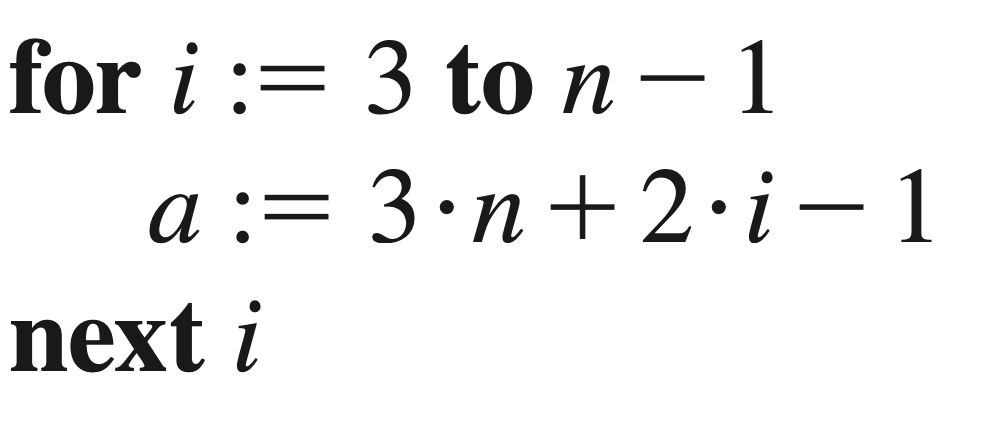
\includegraphics[width=0.3\textwidth]{images/epp_hw_6}%
%\hfill
%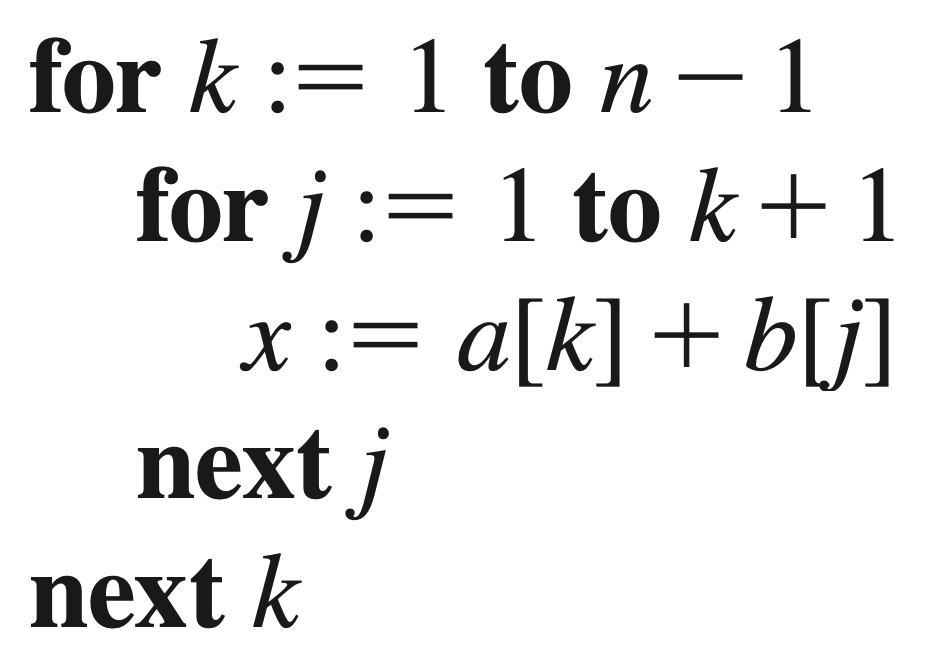
\includegraphics[width=0.3\textwidth]{images/epp_hw_11}%
%\hfill
%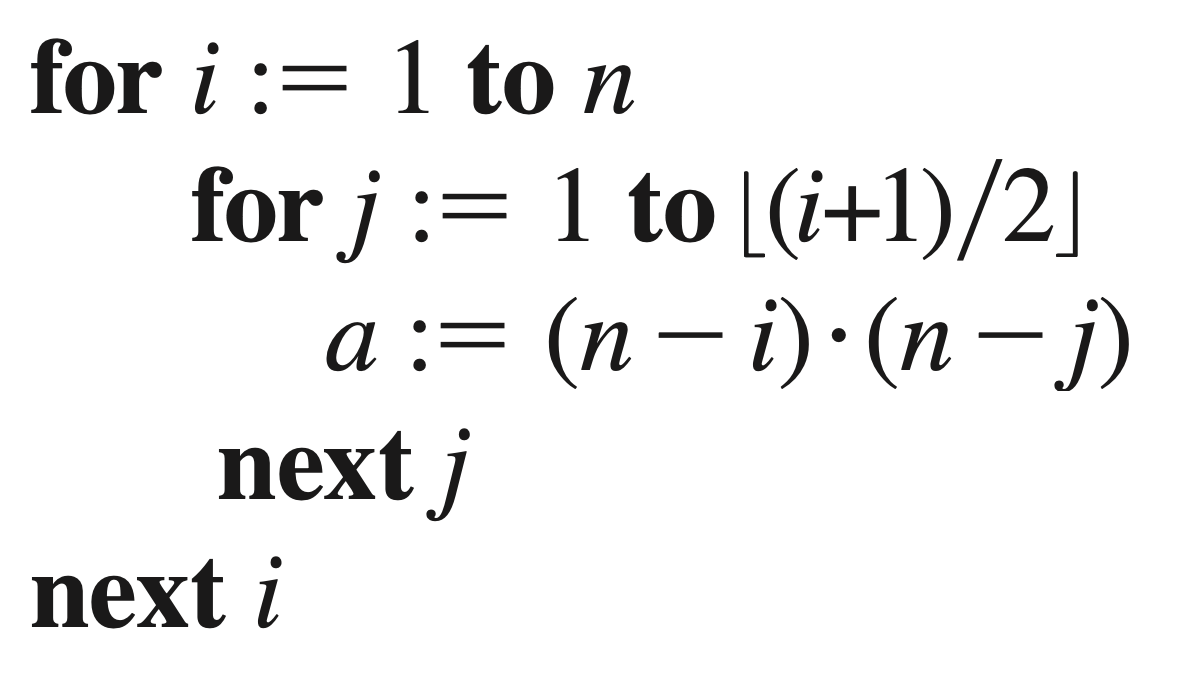
\includegraphics[width=0.3\textwidth]{images/epp_hw_17}% 


\centering
\begin{minipage}{0.3\textwidth}
    \centering
    \small Segment 1 \\
    \vspace{.2cm}
    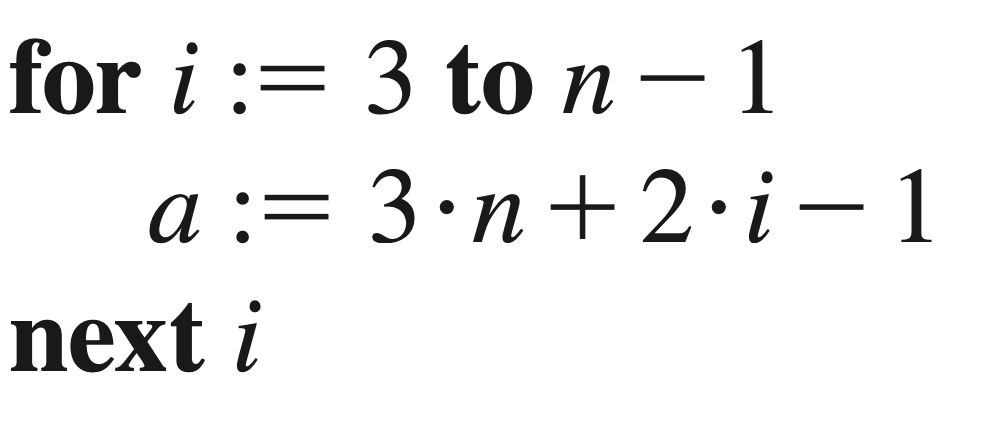
\includegraphics[width=\linewidth]{images/epp_hw_6}% \\
\end{minipage}
\hfill
\begin{minipage}{0.3\textwidth}
    \centering
    \small Segment 2 \\
      \vspace{.2cm}
    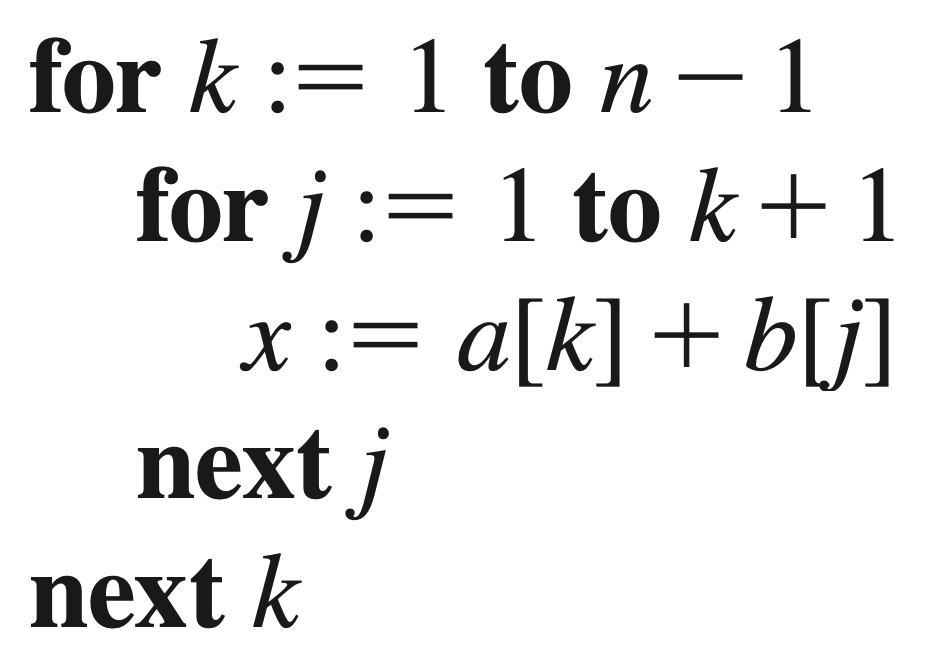
\includegraphics[width=\linewidth]{images/epp_hw_11}% \\
\end{minipage}
\hfill
\begin{minipage}{0.3\textwidth}
    \centering
     \small Segment 3 \\
       \vspace{.2cm}
    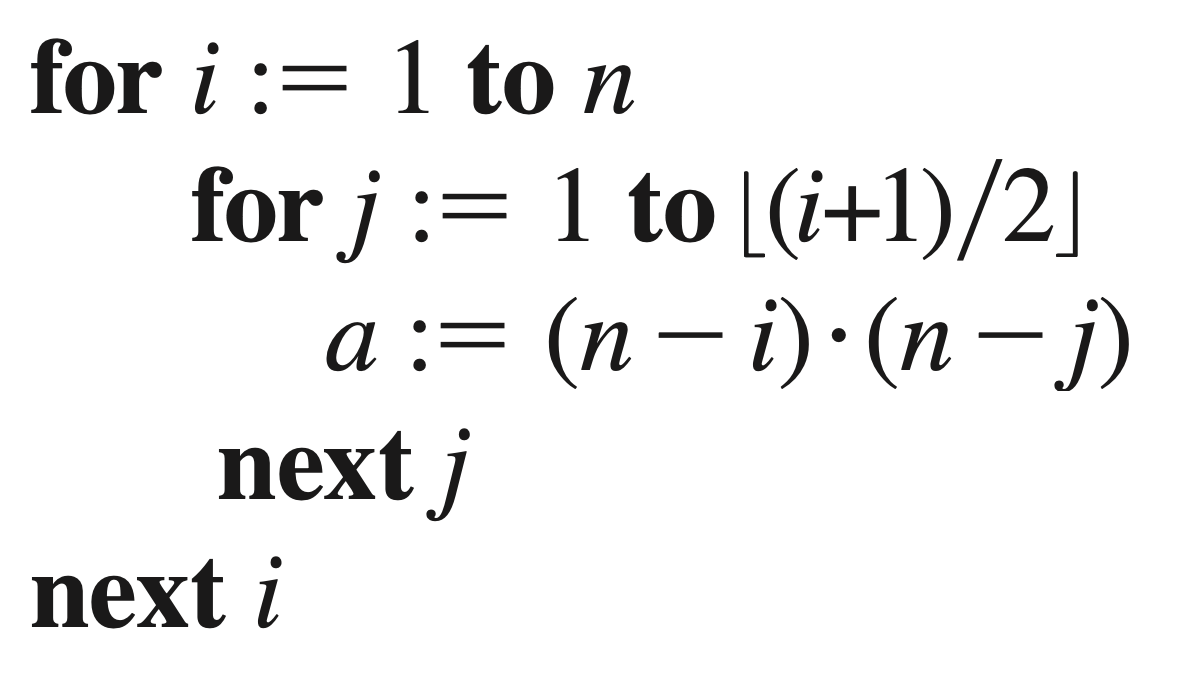
\includegraphics[width=\linewidth]{images/epp_hw_17}%  \\
\end{minipage}


\end{frame}

\end{document}
